%!TEX root = ../thesis.tex
%Adding the above line, with the name of your base .tex file (in this case "thesis.tex") will allow you to compile the whole thesis even when working inside one of the chapter tex files

\chapter{Data Analysis} \label{chap:4}

The complex visibilities outputted from the correlator of a radio interferometer are far from ideal and many additional steps of processing are required before they can be of scientific use. The imperfection of the synthesis radio telescopes (e.g., surface accuracy, receiver noise, gain stability, etc.), the adjustments to the signal (e.g., filter bandpass, etc.), hardware or software failures, poor atmospheric conditions, and the presence of RFI are some of the many sources of visibility corruption that must be accounted for before they can be Fourrier transformed to get the sky brightness distribution. This chapter describes the three main steps involved in reducing any standard radio interferometric data set, namely: data examination and flagging, data calibration, and imaging. In each step we give relevant examples of the data reduction techniques used in \cite{ogorman_2012} and \cite{ogorman_2013}. A general work flow chart is given in Figure \ref{fig:4.1} which highlights the standard procedure required to go from raw visibilities to image analysis and summarizes what will be discussed in this chapter.\\
\\
\begin{figure}[hbt!]
\centering 
          \includegraphics[trim=20pt 270pt 0pt 230pt,clip,scale=0.8]{/home/eamon/thesis/thesis_template/4/cash_flow.ps}
\caption[Radio interferometry work flow chart]{Work flow chart highlighting the general procedure required to go from the raw visibilities outputted by the correlator to a final radio image that can be used for scientific analysis. (Image adapted from the CASA cookbook, NRAO)}
\label{fig:4.1}
\end{figure}

\section{Data Examination and Flagging}\label{sec:4.1}
The Common Astronomy Software Application \citep[CASA;][]{mcmullin_2007} package was used to flag, calibrate, and image the main data sets used in this thesis. CASA is operated through a Python interface and uses a suite of astronomical data reduction tools which have been developed to meet the processing requirements of the large  data sets from the Karl G. Jansky VLA and ALMA. It can also be used to process data from practically all other modern radio synthesis arrays. For synthesis data to be processed in CASA, it must be in a ``measurement set'' format. VLA data is easily transferable into this format using the \textit{importevla} task within CASA. CARMA data files however come in \textit{Miriad} format and need to be first converted into Flexible Image Transport System (i.e., FITS) format within the Miriad \citep{sault_1995} data reduction package. During this process the raw data are smoothed by a Hanning filter (combining adjacent frequency channels with weights 0.25, 0.5, and 0.25) to dampen ringing in the bandpass. Once in FITS format, the data can then be imported into CASA using the \textit{importuvfits} task.

Once the data has successfully been imported into CASA the \textit{listobs} task can be used to get a summary of the data set allowing the user to make sure the observing track contains the requested sources at the correct times. At this point it is also a good idea to check any observing logs which are created on site during the observation by the array operators. These logs usually contain important information about the specific track such as non-operational antennas, unavailable receivers, weather conditions etc., and such data will need to be treated appropriately during calibration or flagged at this stage. The \textit{plotms} task, which is a GUI-style plotter, can then be used to obtain X-Y plots of visibility data. A good visual overview of the observation track is obtained by plotting all the source visibility amplitudes as a function of time. Averaging the data over time/channels/baselines often alerts the user of obvious bad data, which can be manually flagged through the \textit{plotms} interface or through the \textit{flagdata} task. An example of such a plot is shown in Figure \ref{fig:4.2} where the visibility amplitudes of three sources in a 1.3\,cm VLA observing track for Aldebaran are displayed against time. The relatively weak target is shown between interleaving scans of the stronger phase calibrator, while the flux calibrator is the scan at the end of the observing track and is the strongest source in this observation. The data has been averaged over all channels and over a time period of x\,s. Some relatively low visibility amplitudes can clearly be seen for all scans of the phase calibrator which can be traced to a single poor performing antenna.

\begin{figure}[hbt!]
\centering 
\includegraphics[trim=20pt 270pt 0pt 230pt,clip,scale=0.5]{/home/eamon/thesis/thesis_template/4/cash_flow.ps}  
\caption[]{}
\label{fig:4.2}
\end{figure}

Another important way to represent the data at this stage of the flagging process is to plot the visibility amplitude of each of the sources as a function of $u-v$ distance or baseline length (i.e., $\sqrt{(u^2 + v^2)}$). The amplitude distribution should be relatively constant as a function of $u-v$ distance for the phase calibrator (i.e., a point source) and will fall off with increasing baseline length if the flux calibrator is resolved. Plotting the data in this format often results in extreme points at certain baselines which can then often be traced back to poorly behaving antennas or baselines. There is also some flagging which can be carried out based in part on a priori information. Antennas in very compact configurations can partially block the incoming RF signal to other antennas which is often referred to as antenna shadowing. This was not a problem in our VLA B configuration observations but some data obtained in the more compact CARMA configurations had to be flagged as a result of this shadowing. At the time our VLA observations took place, every observing track (i.e., scheduling block) needed to commence with at least a one minute \textit{dummy scan} to facilitate the correlator setup. We subsequently flagged these scans as they contained no useful scientific data. Other a priori flagging was to remove any visibilities with zero amplitudes and to flag the edge channels in the CARMA data sets. Finally visual inspection of each scan was carried out to determine if data at the beginning or end of these scans needed to be flagged. This processes is often referred to as quacking in radio interferometry analysis.

No RFI was present in any of the CARMA data sets and in any of the VLA data sets at wavelengths $\lesssim 3$\,cm (i.e., X, K, Ka, and Q bands). For the 2011 long wavelength ($> 3$\,cm) data the two sub-bands were centered at relatively RFI free regions of the bandpass and only a very small amount of RFI had to be manually flagged. The 2012 wide-band data was taken at 10\,cm (i.e., S band) and 20\,cm (i.e., L band) and many of the sub-band were severely contained with RFI especially at 20\,cm. In Figure \ref{fig:4.3} we plot the visibility amplitude of the flux calibrator 3C286 against frequency for the 2012 wide-band data set at 20\,cm. The upper panel shows the raw data before any RFI has been removed. Some of the sub-bands were so contaminated with RFI that they had to be completely flagged. The remaining sub-bands were initially Hanning smoothed to suppress Gibbs ringing. This action spreads the single-channel RFI into three channels, but importantly removes the effects of some of the worst RFI from a number of channels and allows as much good data to be retained as possible. The \textit{testautoflag} task was then used to conservatively flag RFI from all sources and any remaining RFI was manually flagged. The final result for the flux calibrator is shown in the bottom panel of \ref{fig:4.3} with only some residual RFI still remaining, particularly between 1 and 1.2\,GHz.

\begin{figure}[hbt!]
\centering 
\includegraphics[trim=20pt 270pt 0pt 230pt,clip,scale=0.5]{/home/eamon/thesis/thesis_template/4/cash_flow.ps}  
\caption[]{}
\label{fig:4.3}
\end{figure}

\section{Calibration}\label{sec:4.2}

The role of calibration is to correct the measured visibilities $V'(u,v)$ to approximate as closely as possible the true visibilities $V(u,v)$. As discussed in Chapter \ref{chap:2}, the true visibilities are related to the sky brightness via the Fourier transform:
\begin{equation}
V_{ij}(t) = \int A(l,m) I(l,m) \mathrm{exp}[-i2\pi(u_{ij}(t)l + v_{ij}(t)m)]	dl	dm 
\end{equation}
where $i,j$ represent the discrete sampling of the antennas $i$ and $j$ at time $t$. The term $u_{ij}(t)l + v_{ij}(t)m$ is the geometric phase difference produced by the geometric path length difference between antenna $i$ and antenna $j$ from the source (or part of) at location ($l,m$) relative to the phase center. The relationship between the measured visibility and the true visibility on a baseline between antennas $i$ and $j$ may be expressed as
\begin{equation}
V_{ij}' =  J_{ij}V_{ij}
\end{equation}
where $ J_{ij}$ represents the accumulation of all corruptions affecting baseline $ij$. This equation is known as the Hamaker-Bregman-Sault Measurement Equation \citep{hamaker_1996}. The most important of the effects contained in $J_{ij}$ are antenna-based and arise from the measurable physical properties of individual antenna elements or the measurable physical conditions in the atmosphere above them. Thus, an array of $N$ antennas forming $N(N-1)/2$ baselines can usually be adequately calibrated through the determination of only $N$ factors.

For the purpose of the work presented in this thesis, the Measurement Equation can be written as
\begin{equation}
V_{ij}'(u,v,\nu) = b_{ij}(t)[B_{i}(\nu ,t)B_{j}^{*}(\nu ,t)](t)g_{i}(t)g_{j}(t)V_{ij}(u,v,\nu)e^{i[\theta _{i}(t) - \theta _{j}(t)]}
\end{equation}
where
\begin{itemize}
\item $g_{i}$ and $\theta _{i}$ are the amplitude and phase portions of the complex gain which are usually determined separately in the calibration process and may change over the observation period with temperature, atmospheric conditions, etc. 
\item $B_{i}$ is the complex bandpass, the instrumental response as a function of frequency, $\nu$ and may also vary over time.
\item $b_{ij}(t)$ is the baseline term and is important shortly after a configuration change when antenna positions may not be known well.
\end{itemize}
The general calibration strategy is then to derive a series of scaling factors from both the phase and flux calibrators, which are then collectively applied to the science target. 

%In order to calibrate the data, we solved for the complex gains of the calibration sources while applying the bandpass solution, which was derived from the relevant flux calibrator.  The amplitude gains of the phase calibrators were scaled according to values derived from the flux calibrators using the ``Perley-Butler 2010" flux density standard \citep{2013ApJS..204...19P}. At the time, no Ka or S-band flux density standard models were available so instead for these we used the K and L-band models, respectively, which were scaled according to their spectral indices. The more frequently observed phase calibrators were then used to calibrate the amplitude and phases of the targets. Atmospheric opacity corrections were also applied to the high frequency data sets using the average of a seasonal model (based on many years of measurements) and information from the weather station obtained during the observations.

\section{Imaging}\label{sec:4.3}

%The image cubes were multiscale CLEANed down to the
%3 threshold using natural weighting and were corrected for
%primary beam attenuation. The multiscale algorithm (Rich et al.
%2008) within CASA was set to four unique scales; the largest
%corresponding to the largest structures visible in individual
%channel maps. Each scale was approximately set to three times
%smaller than the preceding scale.
%
%The visibilities were then both Fourier transformed and deconvolved using the CASA \textit{clean} task in multi-frequency synthesis imaging mode, which separately grids the multiple spectral channels onto the \textit{u-v} plane and therefore improves the overall \textit{u-v} coverage. We used natural weighting for maximum sensitivity and the cell size was chosen so that the synthesized beam was about five pixels across. For the high frequencies it was usually sufficient to place just one CLEAN circle around the target source.  For the low frequencies however, the image sizes were usually set to a few times the size of the primary beam so that nearby strong serendipitous sources could be CLEANed thus reducing their sidelobe contamination of the final image. These images were CLEANed interactively, taking sky curvature into account, down to about the $3\sigma$  level with clean boxes placed around sources as they appeared in the residual image. All images were corrected for  primary beam attenuation. 
%
%CLEAN vs MEM vs Multi-scale Clean (for Peter!)
%
%second sources (maps)
%
%Dirty Image, PSF
%
%Show images of calibrators